\section{Actor Models} 

In previous work~\cite{gledhill2013modelinguas} we represented each member of the WiSAR system as a unique directed role graph(DiRG); see Figure 1. As is common
when modeling human-automation interaction we modeled the DiRGs using Mealy state machines which we refer to as Actors~\cite{bolton2013litreview}. However the model did not lend itself well to workload analysis. Converting the actors to Moore machines allowed for greater precision in model validation and workload analysis. While Mealy machines signals are based both on the inputs into a state and the state itself Moore machines restrict changes to the input to state changes. This confines the non-determinism of the model to state changes. By minimizing points of non-determinism we simplify the validation process for the model.

{\sc State why Moore machines are better than Mealy, reminding the reader about the differences between the two.}

\begin{figure}[h]
\center
\setlength{\abovecaptionskip}{1mm}
\setlength{\belowcaptionskip}{1mm}
\setlength{\textfloatsep}{1mm}
\setlength{\floatsep}{1mm}
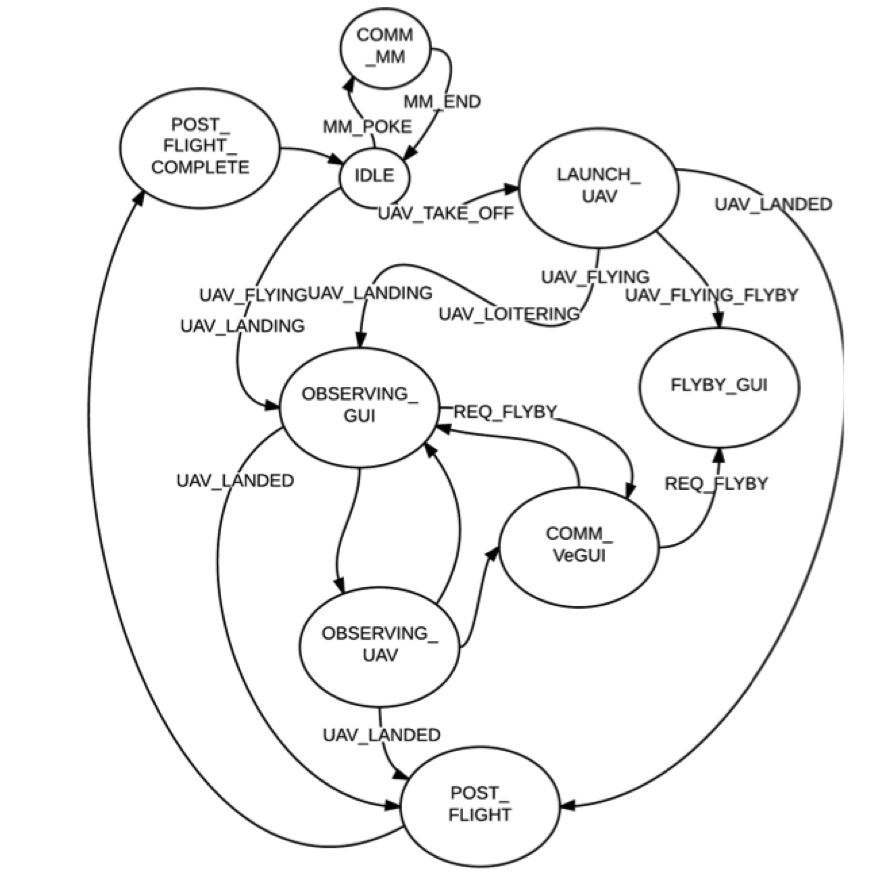
\includegraphics[height=2.4in]{DiRG.png}
\caption{DiRG}
\label{fig:dirg}
\end{figure}

Formally, the actors are modeled as Moore machines as follows:

\begin{equation}
 	Actor = (S, s_0, s_{current}, \Omega_A, \Sigma_A \subset \Phi, \Lambda_A
 	\subset \Phi)
 \label{eq:actor}
 \end{equation}

 \begin{equation}
	State = (T_{enabled}, T_{disabled}) : T_{enabled} \cap T_{disabled} = \emptyset
 \label{eq:state}
\end{equation}

\begin{equation}
\begin{split}
	Transition = (\Omega_{input} \subset \Omega_A, \Sigma_{input} \subset \Sigma_A,\\
	\Omega_{value}^{input}, \Sigma_{value}^{input} \\
	\Omega_{output} \subset \Omega_A, \Lambda_{output} \subset \Lambda_A, \\
	\Omega_{value}^{output}, \Lambda_{value}^{output}, duration)
 \label{eq:transition}
 \end{split}
\end{equation}

{\sc State in a few sentences what these things mean and how we use them.  Take items 1-3 from the Framework Components section in section III.B.}
